\chapter{Configuring the application environment}\label{ch:remote}
\index{Remote computing}

After the local structure and workflow exercises, you may want to adjust the interface, connect to a materials database, or submit work to a configured remote environment. These features serve different purposes: settings connect the application to personal services, remote computing chooses where a workflow runs, and logs and help explain its state and support problem reporting.

This chapter covers everyday settings and chat services before remote submission from the full MATLAB\regmark{} toolbox. Section~\ref{sec:node-resources} covers CPU, process-pool, and GPU settings within a node; the remote sections here choose the execution environment. Standalone and Runtime-based Online users can use node resources as supported by their deployment and refer to the settings, chat, logs, and help sections.

\section{Adjust application settings}

\subsection{Open Settings and save changes}

Click \ui{Settings} in the Environment section of \ui{Home}. General contains language and chat settings. Materials Project contains database access settings. Online environments connected to an account service also provide an Account page.

Click \ui{OK} to save changes. \ui{Cancel} or closing the window discards unconfirmed edits. Reopen Settings to read the saved values and check what is actually in effect.

\subsection{Change the interface language}
\index{Interface language}

\begin{steps}
\item Open \ui{Home → Settings → General}.
\item Select the interface language in the Language section.
\item Click \ui{OK} to save it.
\item Save your project and restart the application.
\item Check that ribbon and panel titles use the new language.
\end{steps}

The language takes effect at the next start. Close and reopen a desktop application. In Online, \ui{Exit KSSOLV Toolbox} only returns temporarily to the portal while the instance keeps running. Save first, then use your platform's sign-out or restart procedure to enter a new instance.

Figure~\ref{fig:settings-language-field} shows the language section of Online General settings with English selected. The message below the field says that the change takes effect at the next start, matching the save-and-restart sequence above.

\begin{figure}[!htb]
\centering
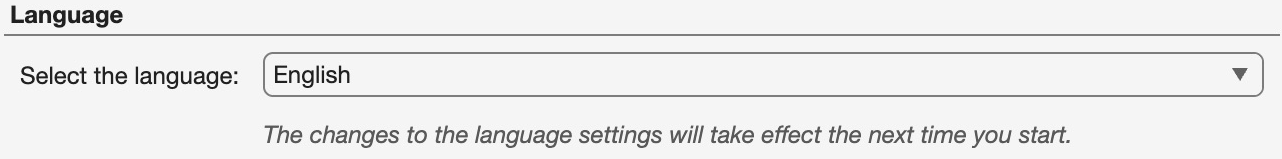
\includegraphics[width=102mm]{publication-assets/crop-290321d16b2310a99270.png}
\caption{The language field in General settings, with English selected.}
\label{fig:settings-language-field}
\end{figure}

\section{Connect a chat service}\label{sec:llm-configuration}
\index{Chat services}

\subsection{Choose a service type}

The Command Window accepts both ordinary commands and questions for a large language model. \ui{OpenAICompatible} uses an OpenAI-compatible API with an endpoint, key, and model supplied by the provider. \ui{Ollama} connects to a running Ollama server and uses models installed there.

Chat can explain terminology, compare parameter purposes, and help organize notes. Models supporting tool calls can also read the current workflow and rename node labels. Chat is optional: structure import, modeling, and DFT calculations work independently.

\begin{table}[!htb]
\centering
\caption{Information needed to connect a chat service.}
\label{tab:llm-connection-fields}
\begin{tabularx}{\linewidth}{lXX}
\toprule
Setting & OpenAICompatible & Ollama \\
\midrule
Address & \ui{API Base URL}, including the provider's required version path, such as \file{/v1}. & \ui{Server URL}, such as \url{http://127.0.0.1:11434} for a local service.\\
Credentials & \ui{API Key} for this base URL. & No API Key field is provided here.\\
Model & \ui{Model Used}: select or enter a model identifier available to your account. & \ui{Model Used}: select or enter a name and tag already installed on the server.\\
Check & \ui{Test Connection} or Refresh retrieves the model list. & \ui{Test Connection} or Refresh retrieves installed models.\\
\bottomrule
\end{tabularx}
\end{table}

Requests originate from the computer running the toolbox. For a desktop application, this is normally your computer. For Online, it is the server or container; the browser's computer does not automatically host the model service.

\subsection{Configure an \headinglatin{OpenAI}-compatible service}

Obtain the base URL, personal API key, and authorized model identifier from your provider. ``OpenAI-compatible'' describes the interface; the service determines the provider and models.

\begin{steps}
\item Under \ui{Home → Settings → General → LLM}, set \ui{Type} to \ui{OpenAICompatible}.
\item Enter the provider's \ui{API Base URL}, retaining its required version path.
\item Enter your personal \ui{API Key}.
\item Click \ui{Test Connection} and wait for the model-list status.
\item Select a model in \ui{Model Used}, or enter its exact identifier as instructed by the provider. Check it and click \ui{OK}.
\item Ask a short conceptual question in the Command Window to check an actual response.
\end{steps}

Figure~\ref{fig:settings-service-fields} shows the configuration fields. Retain the required version path in the base URL and match the model identifier to the service. Use \ui{Test Connection} to retrieve its list.

\begin{figure}[!htb]
\centering
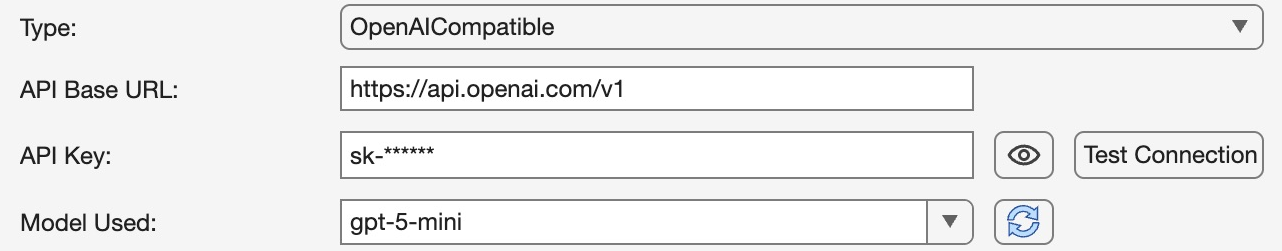
\includegraphics[width=\linewidth]{publication-assets/revision-llm-openai-compatible.png}
\caption{OpenAI-compatible service settings. Base URL, key, and model are separate fields; the key is masked.}
\label{fig:settings-service-fields}
\end{figure}

Use the provider's API base URL without specific endpoints such as \file{/chat/completions} or \file{/models}. Retain a required \file{/v1} suffix. The application appends model-list and chat paths itself and rejects base URLs already containing those specific endpoint paths.

The key is normally masked. Reveal it briefly with the display control if correction is necessary, then hide it again. To remove a saved OpenAI key, first choose a service that does not use it, clear the field, and click \ui{OK}. With OpenAICompatible still selected, Settings requires a usable key. Keep credentials hidden in screenshots and screen sharing.

\subsection{Configure \headinglatin{Ollama}}

Ollama must already be running at an address reachable by the application. Desktop users may use a local service; Online users need an address reachable from the server. Requests come from the toolbox host.

\begin{steps}
\item Set \ui{Type} to \ui{Ollama}.
\item Enter the service root in \ui{Server URL}, without \file{/api/tags} or another endpoint path. The usual local address is \url{http://127.0.0.1:11434}.
\item Click \ui{Test Connection} and wait for the server's model list.
\item Select an installed model under \ui{Model Used}, or enter its complete name and tag, then click \ui{OK}.
\item Ask a short question in the Command Window and check the status and response.
\end{steps}

In Online, \file{localhost} and \file{127.0.0.1} refer to the server or container running the toolbox, not to Ollama on your laptop. For a shared service, enter the address supplied by your deployment. Typing a model name does not download it to the server. Install the model and start its service in the hosting environment first.

\begin{figure}[!htb]
\centering
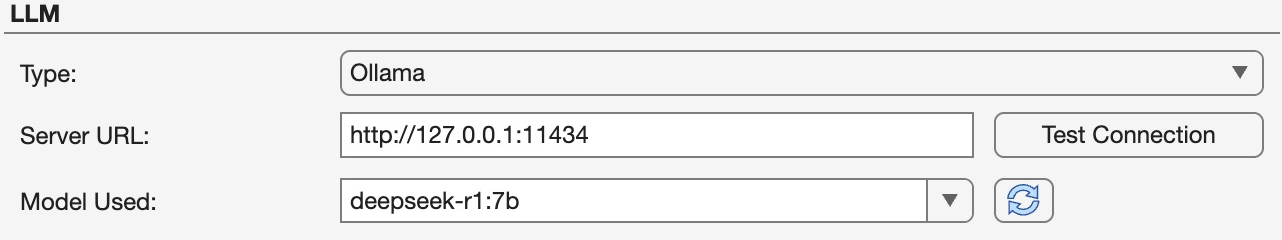
\includegraphics[width=\linewidth]{publication-assets/revision-llm-ollama.png}
\caption{Ollama server address and model settings.}
\label{fig:llm-ollama-live}
\end{figure}

\subsection{Refresh the model list}

\ui{Test Connection} and the refresh icon beside the model perform the same check: retrieving the model list from the current address. OpenAI-compatible services use \file{/models}; Ollama uses \file{/api/tags}. A nonempty list produces a connection-success message and model count. Check actual text responses and tool support by asking a question.

Refresh after changing an address or key, then inspect \ui{Model Used}. During testing, the button changes to \ui{Stop Test} to end the wait. The model field also accepts manual entry. If the service has no enumerable list but its provider gives an exact model identifier, enter and save it, then test a short question. The list check may still report that no models were found.

For authentication errors, check that the address and key belong to the same service. For missing endpoints, check the base URL and version path. For timeouts or secure-connection messages, check connectivity from the toolbox host. If list retrieval succeeds but chat fails, inspect model permissions, the chat endpoint, and tool-call support instead of repeatedly refreshing. A message that the distribution lacks chat components means you need an environment providing them; the structure and DFT tutorials are unaffected.

\subsection{Ask a question in the Command Window}\label{sec:chat-use}

Commands and chat share one input area and are distinguished by their prefix. Enter MATLAB\regmark{} expressions directly. One dollar sign starts a question using the existing conversation context; two dollar signs make an independent request without that history. The signs are part of the input; no separate chat page is needed.

\begin{table}[!htb]
\centering
\caption{Commands and questions in the shared input area.}
\label{tab:command-chat-prefix}
\begin{tabularx}{\linewidth}{lX}
\toprule
Input & Effect \\
\midrule
\texttt{2 + 3} & Evaluates a MATLAB\regmark{} expression and displays its result.\\
\texttt{\$} followed by a question & Asks the model using context from earlier successfully completed turns.\\
\texttt{\$\$} followed by a question & Makes an independent request without reading or appending to the retained conversation context.\\
\bottomrule
\end{tabularx}
\end{table}

\begin{steps}
\item Confirm service and model settings, open the Command Window, and wait for input to become available. Enter \literalinput{2 + 3} and press Enter to see where ordinary output appears.
\item Enter \literalinput{$ Explain the plane-wave cutoff energy} and press Enter. Observe the waiting status and streamed response.
\item Follow up with \literalinput{$ Why do I also need to test k-point convergence} to use the same conversation.
\item For a separate question, enter \literalinput{$$ Explain the three components of fractional coordinates}. This does not clear the earlier context; a later single-dollar question can still use it.
\item Keep useful explanations in your notes, then return to modeling or calculation.
\end{steps}

The application creates the selected chat client on the first question. Watch its waiting status and streamed reply; the final status may identify the model actually returned by the service. Wait for one response to finish before asking the next question.

Replies can contain text, code blocks, and mathematical expressions. Displayed code is not executed automatically. Check its variables and inputs before submitting any command separately without a dollar sign. Include the relevant structure, calculation conditions, and numerical values when asking a specific question.

\begin{figure}[!htb]
\centering

\includegraphics[width=108mm]{publication-assets/revision-llm-question-input.png}
\caption{A question entered in the Command Window before sending. The leading dollar sign distinguishes chat from an ordinary command.}
\label{fig:llm-input-live}
\end{figure}

\subsection{Let the model inspect and organize a workflow}\label{sec:chat-workflow-tools}

Tool-capable models can request two application operations: read the current graph's nodes and connections through \texttt{getCurrentGraph}, and change a specified node label through \texttt{changeNodeLabel}. These tools do not create structures, change calculation parameters, run calculations, or read all numerical results in the project.

OpenAI-compatible requests include both tool definitions, so the provider and model must support that tool-call format. Ollama exposes tools according to the model capabilities reported by its service. A model without tools can still answer ordinary text questions. Check both the conversation and canvas to see whether a tool ran.

\begin{steps}
\item Save the project and activate an existing workflow.
\item Enter \literalinput{$ Read the current workflow and describe its node labels and connection order}. A tool-capable model can base its answer on the actual graph.
\item Compare its labels with the canvas. If the reply is generic, explicitly request the current workflow. If actual graph information is still absent, check model tool support.
\item Identify an unambiguous node, such as the workflow's only SCF node. Enter \literalinput{$ Change the SCF node label in the current workflow to "Electronic self-consistency"}. With several matching nodes, supply the original label to identify the target first.
\item Check the changed label on the canvas, open the node to confirm that its task remains SCF, and save.
\end{steps}

Renaming changes only the canvas label. It does not turn another task into SCF or rerun the solver. Inspect the canvas for the actual change. Continue using node configuration and graph editing for cutoffs, grids, and execution order as described elsewhere.

\subsection{Chat after changing settings}

Clicking \ui{OK} in Settings rebuilds an existing chat client, so the next question starts a new context. Retain any explanations you need even if you are merely confirming unchanged settings. \ui{Cancel} does not apply edits. Keep important explanations, notes, and conclusions in your calculation record alongside project inputs and results.

If a streamed response disconnects, the interface reports an incomplete or failed turn. A failed turn does not replace previously retained complete context; check the connection and ask again. The incomplete reply remains visible. If a tool already changed a label during that turn, inspect the canvas to check the actual state.

\section{Set up \headinglatin{Materials Project} access}
\index{Materials Project}

Materials Project is one source of structures. Its import tool needs personal access settings. Importing a local CIF or XYZ does not.

\subsection{Save an API key}

\begin{steps}
\item Open \ui{Settings → Materials Project}.
\item Click \ui{View My API Key} to open your API page in the browser.
\item Sign in as required by the database website and copy your own key.
\item Return to the application, enter it in API Key, and click \ui{OK}.
\item Choose \ui{Home → Structure → Import structure from Materials Project...}.
\end{steps}

Settings stores service credentials, not a particular structure. Searches and downloads originate from the toolbox host. In Online, check that the server can reach the database.

After saving access settings, use Section~\ref{sec:mp-search} to search by periodic-table selection, formula, or MP ID. Its silicon example shows the results table, mp-149 selection, and imported 3D structure.

\section{Understand remote computing}

\subsection{Online and remote clusters}

The toolbox in full MATLAB\regmark{} provides a \ui{Remote} menu to submit the current workflow to another MATLAB\regmark{} environment or cluster. The standalone application and Runtime-based Online do not show this menu. The following configuration and submission procedures apply to the full MATLAB\regmark{} toolbox.

Online already runs on a server and does not require browser users to configure SSH first. The location of the workspace and submission to a cluster are separate matters: one identifies where the application runs, and the other sends a task to a chosen computing environment.

A remote job record contains the workflow, submission target, status, and output. Successful submission means the target accepted the job; it may still be queued or encounter problems during execution. After completion, fetch results into the project and save it.

\subsection{Check location and resources separately}

The \ui{Resources} panel in Section~\ref{sec:node-resources} chooses Serial, a process pool, or GPU on the execution machine. Remote configuration chooses the machine, cluster profile, and retrieval method. Enabling a node pool does not submit a cluster job; selecting a cluster does not make every node parallel.

Online may disable the Home \ui{Parallel} button while still offering task-specific node resources. Actual capability depends on the server's components, pools, and GPUs. Cluster submission here applies to the Remote menu in full MATLAB\regmark{}.

\subsection{Choose an execution mode}

\begin{table}[htbp]
\centering
\caption{Remote execution modes.}
\begin{tabularx}{\linewidth}{lX}
\toprule
Mode & Environment \\
\midrule
Standard & Local MATLAB\regmark{} submits through MATLAB\regmark{} Parallel Server and Slurm; local and remote calculation components use the same release.\\
Bridge & Remote MATLAB\regmark{} submits through its own cluster profile; that MATLAB\regmark{} and its workers use the same release.\\
Mirror & Ordinary MATLAB\regmark{} on one remote node; MATLAB\regmark{} Parallel Server is not required.\\
Cloud & An existing, configured, and validated cloud MATLAB\regmark{} cluster profile.\\
\bottomrule
\end{tabularx}
\end{table}

Prefer a mode already validated by your institution. Mirror can suit an ordinary single-node MATLAB\regmark{} environment. For Parallel Server with Slurm, follow administrator guidance on Standard or Bridge. Cloud requires a prepared profile; selecting it does not provision a new cloud cluster.

Remote execution requires the corresponding MATLAB\regmark{} products and licenses, with Parallel Computing Toolbox locally. Administrators prepare version compatibility and cluster installations. Check that your selected configuration matches the actual environment.

\section{Create a cluster configuration}
\index{Cluster configurations}

\subsection{Gather remote information}

Ask the administrator for the host, authentication method, remote MATLAB\regmark{} root, and writable job directory. Also obtain a profile name if used, or Slurm partition, account, QoS, and wall-time requirements.

Name configurations by purpose, such as ``Materials cluster,'' rather than ``Server 1.'' Login nodes, compute nodes, and shared storage may differ. Use supplied site information rather than guessing remote paths from your local computer.

\subsection{Enter the configuration}

\begin{steps}
\item Open \ui{Home → Remote → Configure Remote Clusters…}.
\item Click \ui{Add}, enter a name, and choose the execution mode.
\item On \ui{Connection}, enter host and authentication details as instructed.
\item On \ui{Compute}, enter the mode's MATLAB\regmark{} root, profile, job directory, and resources.
\item Choose whether to attach the current toolbox or use a cluster-installed copy.
\item Click \ui{Test Connection} and inspect its status.
\item Use \ui{Probe Resources} if needed, check the discovered values, and click \ui{Save}.
\end{steps}

The MATLAB\regmark{} root is the installation directory, not \file{bin/matlab}. Use a writable remote job directory visible to the relevant compute nodes. Respect site resources and licenses when choosing workers; do not simply enter the machine's total core count.

\ui{Test Connection} checks connection and login steps; a profile-based configuration may also run a minimal test job. \ui{Probe Resources} discovers remote MATLAB\regmark{} and resource information. They serve different purposes: connection testing does not replace resource discovery, and discovered values are not saved automatically.

\subsection{Match job resources to node limits}

\ui{Pool workers} requests a parallel pool for each remote job. Its value must lie between 0 and the configuration's Maximum workers. A value of 0 requests no job pool. This differs from a node's maximum-process limit: submission prepares the pool, while the node constrains the pool it accepts.

For NSCF and DOS limited to 2 processes with 1 CPU thread each, request 2 pool workers in a supporting remote mode and ensure remote computational threads do not exceed 1. An existing 4-worker pool conflicts with a node limit of 2; adjust the pool or node settings. An existing compatible 1-worker pool also meets the limit, but uses only 1 worker.

A job already running on a remote worker cannot automatically create a nested pool inside a node. Prepare a suitable pool in advance for job-submission modes such as Standard and Bridge. Mirror execution in an ordinary remote MATLAB\regmark{} process must also respect that machine's local process-pool capabilities. GPU mode requires a supported GPU on the execution machine; your computer displays the interface while the remote GPU performs the numerical work.

The node time-limit field does not stop a calculation. Scheduler wall time is a separate setting governed by site policy. Save the remote configuration and project, and record pool size, node limits, and scheduler conditions together for timing comparisons.

\subsection{Choose how to deploy the toolbox}

Attach Current Toolbox transfers the current toolbox to the target, useful when a matching version is not already installed. The first transfer of a version may take longer; later jobs can reuse prepared code.

Cluster Installed uses an administrator-maintained installation. Enter its root and confirm version compatibility. Centrally managed environments usually specify which option to use; do not modify shared application directories yourself.

A post-login script initializes the environment, for example by loading a site's MATLAB\regmark{} module. Command templates and prompt rules address special routing or additional authentication; fill them only when the administrator requires them. Keep ordinary direct connections simple when they work.

\section{Exercise: submit and retrieve a calculation}
\index{Remote jobs}

Use a completed small silicon workflow with the earlier settings. Focus on submission and result management without changing material and method at the same time.

\subsection{Save and choose the target}

\begin{steps}
\item Open the existing project and workflow; check the structure, connections, and main settings.
\item Save and give the workflow a recognizable name.
\item Choose \ui{Home → Remote → Use Remote Computing} and select a saved configuration such as ``Materials cluster.''
\item Use \ui{Test Current Cluster} if another connection check is needed.
\item Click \ui{Run}, wait for the submission message, and record the job ID.
\end{steps}

Successful submission creates a job record. \ui{Do Not Use} means execution in the current MATLAB\regmark{} environment. Check target names when switching so that a comparison run is not sent to the wrong environment.

\subsection{Track the job}

\begin{steps}
\item Open \ui{Home → Remote → Remote Jobs and Results…}.
\item Select the new job and check its workflow, cluster, and submission time.
\item Click \ui{Refresh} to inspect queued, running, or completed status.
\item Click \ui{View Diary} and read calculation output for parameter and convergence messages.
\item If task settings need correction, use \ui{Cancel Job} first, then edit the workflow and resubmit.
\end{steps}

Unknown means the state cannot currently be read reliably, not that calculation necessarily failed. Check the network and scheduler before refreshing. An empty Diary may mean the job has not started; consider submission time and queue state together.

\subsection{Fetch and import results}

\begin{steps}
\item Confirm completion and choose \ui{Fetch and Import}.
\item Wait for transfer and import confirmation.
\item Find the corresponding data or figures in the Project Browser.
\item Inspect convergence, energy, and related results using the earlier chapters' checks.
\item Save the project to retain the fetched results in its \file{.ks} file.
\end{steps}

If the job was already imported, the application reports that the results exist rather than adding duplicates. Import needs the corresponding workflow in the current project. Retain the submitting project and do not delete or replace the whole workflow before retrieval.

Check SCF convergence, energies, and parameters after fetching. If remote and local results differ, compare structures, pseudopotentials, and node settings before attributing differences to the computing environment.

\subsection{Organize job records}

\ui{Clean Local Bundle} removes the local transfer bundle without canceling the remote job. \ui{Delete Record} removes only its local record, not the remote working directory. Use \ui{Cancel Job} to stop a calculation.

Existing jobs retain the information identifying their submission environment. Editing a configuration later does not move old jobs to another server. Fetch required results and save the project before cleaning up unneeded transfer contents.

\section{Use the remote Command Window}

\ui{Run Command Window Commands Remotely} opens a persistent MATLAB\regmark{} session using the selected direct SSH configuration. It is independent of workflow submission and suits short environment checks or interactive operations. A profile-only configuration without direct connection details cannot use it.

\begin{steps}
\item Select a validated direct configuration.
\item Open the Command Window and enable \ui{Run Command Window Commands Remotely}.
\item Enter a short check such as \texttt{version}.
\item Confirm remote execution from the \texttt{[remote]} input/output prefix.
\item Disable remote execution afterward to return to ordinary commands.
\end{steps}

Commands in the same remote session share a base workspace. Changing targets, disabling remote commands, or closing the Command Window ends that session. Save lasting data to appropriate files. Use workflows for scientific steps you intend to repeat.

\section{Find help}
\index{Logs and help}

\subsection{Check the current state}

The Resources section provides \ui{Documentation}, \ui{Community}, and \ui{Help}. \ui{About KSSOLV} shows product information, and \ui{Check for updates} reports new versions. Installation follows the distribution's or deployment's update procedure. Online external links open in the browser; return to the workspace to continue editing.

When reporting a problem, identify whether it occurs during import, parameter entry, execution, retrieval, or display. State the step, what you see, and what you expected instead of simply saying that it does not run.

\subsection{Collect logs}

\begin{steps}
\item Save the project and note the application version and edition.
\item Choose \ui{Open Log} from \ui{Help}.
\item Desktop opens the log in the system's default application. Online shows it within the page, with refresh and full-file download actions.
\item Locate messages around the time of the issue and retain the relevant portion.
\item Prepare a clear screenshot and a small reproducible project.
\item Click \ui{Request Support}, then compose and send the report in your mail application.
\end{steps}

\ui{Request Support} opens a draft with a subject. Add your explanation and attachments, review them, and send it yourself. If no default mail application is configured, use another contact route provided by the resources. Check screenshots and logs for personal credentials before sharing.

\subsection{Read license and update information}

Choose \ui{Home → Help → License} to read the current product license. Follow the release's license and deployment terms for citation, distribution, or use in another environment.

\ui{Check for updates} reports available versions; \ui{About KSSOLV} identifies the running version. Save before updating and follow the platform instructions in Chapter~\ref{ch:install}. Browser deployments are updated by their administrators. A grayed-out Examples or extension entry is unavailable; the supplied examples can still be imported from this manual's examples directory.

\subsection{A useful diagnostic sequence}

For chat authentication failures, check the base URL, key, and model permissions. For an empty model list, check that the service provides available models. For remote connection failures, inspect authentication and post-login scripts. For submission failures, inspect partition, account, profile, and version requirements. If a completed job cannot be imported, open the original submitting project and read Diary and import messages.

Keep each check focused rather than changing many settings together. Once resolved, rerun a minimal exercise before returning to a larger project. Save the final configuration and parameters with the project and your notes for reproducibility.
